\documentclass{article}

\usepackage{mmacells}

\usepackage{pandekten}
\usepackage{dashrule}

\makeatletter
\newcommand*{\shifttext}[1]{%
  \settowidth{\@tempdima}{#1}%
  \hspace{-\@tempdima}#1%
}
\newcommand{\plabel}[1]{%
\shifttext{\textbf{#1}\quad}%
}
\newcommand{\prule}{%
\begin{center}%
\hdashrule[0.5ex]{.99\linewidth}{1pt}{1pt 2.5pt}%
\end{center}%
}

\makeatother

\newcommand{\minusbaseline}{\abovedisplayskip=0pt\abovedisplayshortskip=0pt~\vspace*{-\baselineskip}}%

\setlength{\parindent}{0pt}

\title{Assignment 2}
\author{Ze Chen}

\begin{document}

\maketitle

\plabel{1 (a)}%
Fixing $u_{2n}$, the minimal of $t m^2 / 2 + u_{2n} m^{2n}$ is at $m \propto (-t)^{1/(2n-2)}$ with value $\propto (-t)^{2n/(2n-2)}$.
Therefore, the singular behavior is given by
\[ C_{\text{s}} \sim (-t)^{2n/(2n-2) - 2}. \]
The flucuation contribution is still
\[ C_{F} \sim (-t)^{d/2-2} \]
since around the saddle point the model has approximately the Gaussian form.
For there two contributions to be comparable, we find
\[ \frac{n}{n-1} - 2 = \frac{d}{2} - 2 \]
and therefore the critical dimension $d = (2n)/(n-1)$.

\plabel{(b)}%
The gradient terms doesn't affect the saddle point and therefore doesn't affect $C_{\text{s}}$.
\par
By expanding with respect to $\delta m$ to the second order, the gradient terms should not affect the mass.
They do affect the propagator and change the propagator by
\[ \frac{1}{p^2 + m^2} \mapsto \frac{1}{\cdots + (?)\cdot p^4 + p^2 + m^2} \]
but they don't affect the behavior of $C_{F}$ in terms of $t$ by dimensional analysis since
\[ \int \dd[d]{p} \frac{1}{(t + p^2 + \cdots)^2} \sim t^{d/2-2}. \]

\prule

\plabel{2 (a)}%
If we assume that $R_b$ is linear and diagonal, then $t' = R_b^{(t)}(t)$ and $h' = R_b^{(h)}(h)$.
By defining $R_{b^{-1}} = R^{-1}_b$ we find two one-dimensional representations of the abelian group $\mathbb{R}^\times_{>0}$ given by $b\mapsto R_b^{(t)}$ and $b\mapsto R^{(h)}_b$, i.e. they have to be $R^{(t)}_b = b^{y_t}$ and $R^{(h)}_b = b^{y_h}$.
Pluggin these into eq (3) in the question we find eq (4) in the question.

\plabel{(b)}%
Since
\[ f(t,h) = b^{-d} f(t b^{y_t}, h b^{y_h}), \]
differentiating with respect to $h$ we find
\begin{align*}
    (\partial_2 f)(t,h) = b^{-d + y_h} (\partial_2 f)(t b^{y_t}, h b^{y_h}), \\
    (\partial_2 \partial_2 f)(t,h) = b^{-d + 2y_h} (\partial_2 f)(t b^{y_t}, h b^{y_h}).
\end{align*}
Up to some constant factors,
\begin{align*}
    f(t,0) &= t^{d/y_t};\quad f(0,h) = h^{d/y_h}, \\
    (\partial_2 f)(t,0) &= t^{(d-y_h)/y_t};\quad (\partial_2 f)(0,h) = h^{d/y_h - 1}, \\
    (\partial_2\partial_2 f)(t,0) &= t^{(d-2y_h)/y_t};\quad (\partial_2\partial_2 f)(0,h) = h^{d/y_h - 2}.
\end{align*}
That is, $f$, $\partial_2 f$, and $\partial_2\partial_2 f$ have the simplest form that satisfies the scaling.
\begin{align*}
    \eval{c}_{h=0} &\sim T \pdv[2]{f}{t} \sim t^{d/y_t - 2} \Longrightarrow \alpha = 2-d/y_t, \\
    \eval{m}_{h=0} &\sim \eval{\partial_2 f}_{h=0} \sim t^{(d-y_h)/y_t} \Longrightarrow \beta = \frac{d-y_h}{y_t}, \\
    \eval{\chi}_{h=0} &\sim \eval{\partial_2 \partial_2 f}_{h=0} \sim t^{(d-2y_h)/y_t} \Longrightarrow \gamma = \frac{2y_h - d}{y_t}, \\
    \eval{m}_{t=0} &\sim \eval{\partial_2 f}_{t=0} \sim h^{(d-y_h)/y_h} \Longrightarrow \delta = \frac{y_h}{d-y_h}, \\
    \eval{\xi}_{h=0} &= \xi(t,0) = t^{-1/y_t} \xi(t\cdot t^{-1/y_t\cdot y_t}) \sim t^{-1/y_t} \Longrightarrow \nu = \frac{1}{y_t}.
\end{align*}
Eliminate $y_t$ and $y_h$.
\begin{mmaCell}[morefunctionlocal={t,h}]{Input}
Eliminate[\{t \mmaUnd{\(\pmb{\alpha}\)}==2t-d,t \mmaUnd{\(\pmb{\beta}\)}==d-h,t \mmaUnd{\(\pmb{\gamma}\)}==2h-d,(d-h)\mmaUnd{\(\pmb{\delta}\)}==h,t
\mmaUnd{\(\pmb{\nu}\)}==1\},\{t,h\}]
\end{mmaCell}
\begin{mmaCell}{Output}
\(\alpha\)=2-d \(\nu\land\)2 \(\beta\)=d \(\nu\)-\(\gamma\land\gamma\) (\(\delta\)+1)=d (\(\delta\)-1) \(\nu\)
\end{mmaCell}
That is,
\begin{align*}
    \alpha &= 2-d\nu, \\
    2\beta &= -\gamma + d\nu, \\
    \gamma(1+\delta) &= d\nu(\delta - 1).
\end{align*}

\prule

\plabel{3}%
Since
\[ -\beta H = \sum_{i \text{ odd}} \qty[K \sigma_i \sigma_{i-1} + K \sigma_i \sigma_{i+1} + \frac{h}{2}(\sigma_{i-1} + \sigma_{i+1}) + h\sigma_i + 2g], \]
upon averaging at site $j$ for $j$ an odd number,
\begin{gather*}
    e^{-\beta H(\hat{j})} = \exp[\sum_{\substack{i \text{ odd} \\ i\neq j}} \qty[K \sigma_i \sigma_{i-1} + K \sigma_i \sigma_{i+1} + \frac{h}{2}(\sigma_{i-1} + \sigma_{i+1}) + h\sigma_i + 2g]] \times \\
    \qty(\exp[\qty(K+\frac{h}{2})(\sigma_{j-1} + \sigma_{j+1}) + h + 2g] + \exp[\qty(-K+\frac{h}{2})(\sigma_{j-1} + \sigma_{j+1}) - h + 2g]).
\end{gather*}
Therefore,
\begin{align*}
    e^{-\beta H'} &= \prod_{j \text{ odd}} \\
    &\phantom{{}={}}\exp[\frac{1}{4}\log(\frac{\cosh(h+2K)\cosh(h-2K)}{\cosh^2(h)}) \sigma_{j-1} \sigma_{j+1}] \\
    &\phantom{{}={}} \exp[\qty(\frac{h}{2} + \frac{1}{4}\log(\frac{\cosh(h+2K)}{\cosh(h-2K)}))(\sigma_{j-1}+\sigma_{j+1})] \\
    &\phantom{{}={}} \exp[2g + \log(2) + \frac{1}{4}\log({\cosh(h+2K)\cosh(h-2K)\cosh^2(h)})].
\end{align*}
Therefore,
\begin{align*}
    K' &= \frac{1}{4}\log(\frac{\cosh(h+2K)\cosh(h-2K)}{\cosh^2(h)}), \\
    h' &= h + \frac{1}{2}\log(\frac{\cosh(h+2K)}{\cosh(h-2K)}), \\
    g' &= 2g + \log(2) + \frac{1}{4}\log({\cosh(h+2K)\cosh(h-2K)\cosh^2(h)}).
\end{align*}
The flow is plotted below.
The horizontal axis is $K$ and the vertical axis is $h$.
Lines are flowing to the left.
\begin{center}
    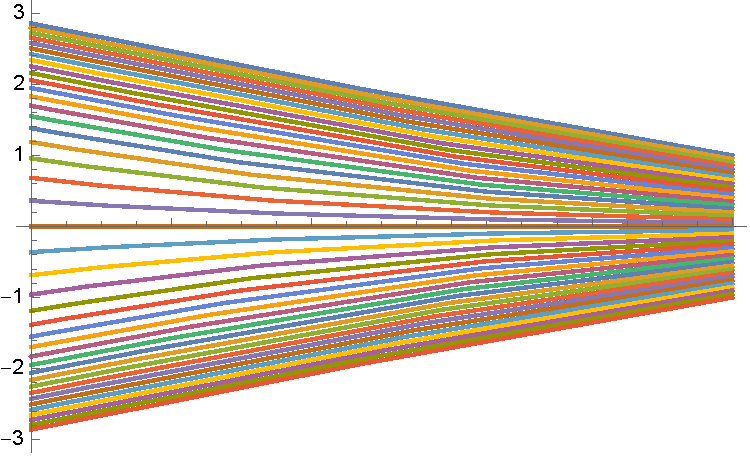
\includegraphics[width=0.5\textwidth]{img/Q3.pdf}
\end{center}
The fixed points are $K=0$, $h\in\mathbb{R}$.
\par
To prove that the prediction is the same as the result using transfer matrix, we should prove the following.
\begin{itemize}
    \item At the fixed point their $Z$ are identical.
    \item $Z_N e^{g N}$ equals $Z'_{N/2} e^{g' N/2}$ under 
    \[ (K,h,g) \mapsto (K',h',g'), \]
    where $Z_N$ and $Z_{N/2}$ are given by the transfer matrix method, for parameters $(K,h)$ and $(K',h')$, respectively.
\end{itemize}
The first statement is clear.
To prove the second statement, it suffices to prove that under $(K,h) \mapsto (K',h')$, the eigenvalues of
\[ T^2 = \begin{pmatrix}
    e^{h+K+g} & e^{-K+g} \\
    e^{-K+g} & e^{-h+K+g}
\end{pmatrix}^2 \]
equals to that of
\[ T' = \begin{pmatrix}
    e^{h'+K'+g'} & e^{-K'+g'} \\
    e^{-K'+g'} & e^{-h'+K'+g'}
\end{pmatrix}. \]
For this, it suffices to prove that $\det(T^2) = \det(T')$ and $\tr(T^2) = \tr(T')$.
The first equation requires
\[ 2 e^{4g} \sinh^2(2K) = e^{2g'} \sinh(2K'). \]
The second equation requires
\[ e^{2(g - K)}(1+e^{4K} \cosh(2h)) = e^{g'+K'}\cosh(h'). \]
These can be verified by plugging in the expressions.
\par
Both results predicts no phase transition.

\plabel{4}%
If the magnetic field is nonzero, then for each block,
\[ Z_0(K,\sigma_I) = 3e^{-K + B\sigma_I} + e^{3K + 3B\sigma_I}. \]
We require that
\[ 3e^{-K + B\sigma_I} + e^{3K + 3B\sigma_I} = e^{\text{const.} + B'_1 \sigma_I}. \]
Therefore
\[ B'_1(K,B) = \frac{1}{2}\log\qty(\frac{3 e^{B-K} + e^{3B+3K}}{3e^{-B-K} + e^{3K-3B}}). \]
To get the equation for $K'$ we define
\[ \Phi(K,B) = \frac{2 e^{4 B+4 K}+e^{2 B+8 K}+3 e^{2 B}+2 e^{4 K}}{\left(3 e^{2 B}+e^{4 K}\right) \left(e^{2 B+4 K}+3\right)}, \]
and
\[ \Sigma(K,B) = \frac{\left(e^{4 B}-1\right) e^{4 K}}{\left(3 e^{2 B}+e^{4 K}\right) \left(e^{2 B+4 K}+3\right)}. \]
Then
\[ \langle S^J_3 \rangle_0 = \Sigma(K,B) + \sigma_J \Phi(K,B). \]
Therefore
\begin{align*}
    \langle U_{IJ} \rangle_0 &= 2K  \langle S^J_3 \rangle_0  \langle S^I_1 \rangle_0 \\
    &= 2K \qty(\Sigma(K,B) + \sigma_J \Phi(K,B)) \qty(\Sigma(K,B) + \sigma_I \Phi(K,B)).
\end{align*}
Now we find
\begin{align*}
    B'(K,B) &= B'_1(K,B) + 6\times 2K\cdot \Sigma(K,B) \cdot \Phi(K,B), \\
    K'(K,B) &= 2K \Phi^2(K,B).
\end{align*}
The flow is given below ($K$ horizontal and $B$ vertical).
Lines are flowing away from the critical point.
\begin{center}
    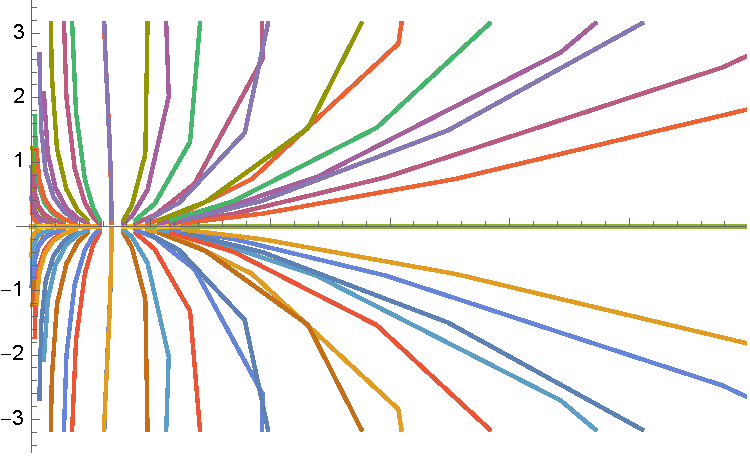
\includegraphics[width=0.5\textwidth]{img/Q4.pdf}
\end{center}

% \bibliographystyle{plain}
% \bibliography{main}

\end{document}
